\documentclass[11pt,a4paper]{article}

% --- Packages ---
\usepackage[utf8]{inputenc}
\usepackage[T1]{fontenc}
\usepackage[margin=1in]{geometry}
\usepackage{graphicx}
\usepackage{xcolor}
\usepackage{amsmath, amssymb, amsfonts}
\usepackage{tikz}
\usepackage{hyperref}
\usepackage{comment}
\usepackage{cleveref}
\usepackage{forest}
\usepackage{subcaption}
\usepackage{listings}
\usepackage{float}
\usepackage{booktabs}
\usepackage{microtype}
\usepackage[bottom]{footmisc}
\usepackage{enumitem}
\usepackage{titlesec}

% --- Formatting ---
\setlist[itemize]{noitemsep, topsep=0pt}
\setlist[enumerate]{noitemsep, topsep=0pt}

\titleformat{\section}{\large\bfseries}{\thesection}{1em}{}
\titleformat{\subsection}{\normalsize\bfseries}{\thesubsection}{1em}{}

% --- Cleveref Setup ---
\crefformat{section}{\S#2#1#3}
\crefformat{subsection}{\S#2#1#3}
\crefformat{subsubsection}{\S#2#1#3}
\crefformat{figure}{Figure~#2#1#3}
\crefformat{table}{Table~#2#1#3}
\crefformat{equation}{Equation~(#2#1#3)}
\crefformat{footnote}{#2\footnotemark[#1]#3}

\crefname{lstlisting}{listing}{listings}
\Crefname{lstlisting}{Listing}{Listings}

% --- Listings Setup ---
\definecolor{codegreen}{rgb}{0,0.6,0}
\definecolor{codegray}{rgb}{0.5,0.5,0.5}
\definecolor{codepurple}{rgb}{0.58,0,0.82}
\definecolor{backcolour}{rgb}{0.95,0.95,0.92}

\lstset{
    language=Go,
    backgroundcolor=\color{backcolour},
    commentstyle=\color{codegreen},
    keywordstyle=\color{magenta},
    numberstyle=\tiny\color{codegray},
    stringstyle=\color{codepurple},
    basicstyle=\ttfamily\small,
    breakatwhitespace=false,
    breaklines=true,
    captionpos=b,
    keepspaces=true,
    numbers=left,
    numbersep=5pt,
    showspaces=false,
    showstringspaces=false,
    showtabs=false,
    tabsize=2,
    frame=single
}

% --- Title Page Info ---
\title{Criticality-Aware Kubernetes}
\author{Giuseppe Capasso \and Emanuele d'Ajello}
\date{Academic Year 2023/2024}

\begin{document}

% --- Title Page ---
\begin{titlepage}
    \centering
    \vspace*{0.5cm}
    
    \begin{minipage}{0.45\textwidth}
        \centering
        
\includegraphics[width=0.8\textwidth]{./figures/unina-logo-1.png}
    \end{minipage}
    \begin{minipage}{0.45\textwidth}
        \centering
        
\includegraphics[width=0.8\textwidth]{./figures/unina-logo-2.png}
    \end{minipage}
    
    \vspace{1cm}
    {\large \textsf{Polytechnic School and Basic Sciences} \\ \textsf{Master's Degree in Computer Engineering} \par}
    
    \vfill
    
    {\Huge \bfseries Criticality-Aware Kubernetes \par}
    \vspace{1.5cm}
    {\Large \itshape Real-Time Industrial Systems Project \par}
    \vspace{1cm}
    {\large Academic Year 2023/2024 \par}
    
    \vfill
    
    \begin{flushleft}
        \large
        \textbf{Students:}\\
        Giuseppe Capasso (ID M63001498)\\
        Emanuele d'Ajello (ID M63001435)
    \end{flushleft}
    
\end{titlepage}

\pagenumbering{roman}
\tableofcontents
\newpage
\pagenumbering{arabic}

% --- Introduction ---
\section*{Introduction}
\addcontentsline{toc}{section}{Introduction}
In a Kubernetes cluster, the Kubelet is responsible for managing the state of a worker node by exchanging information with the control plane. The goal of this project is to analyze the Kubelet's operation to determine if it can be extended to schedule \textit{soft real-time} applications. Specifically, the analysis aims to identify the main factors influencing pod startup latency in Linux environments.

\clearpage

% --- Section 1: Kubernetes ---
\section{Kubernetes}\label{section:kubernetes}
Kubernetes~\cite{KubernetesDocs} is an orchestrator for containerized applications that automates deployment and configuration tasks in cloud environments. A Kubernetes cluster consists of:
\begin{itemize}
    \item \textbf{Data plane}: Contains the \textbf{worker nodes} that execute applications within \textbf{pods}. A pod is the smallest deployable unit in Kubernetes. The component that manages the node's state and resources is the Kubelet, which communicates with the \textit{control plane} to receive instructions and provide status updates on the pods.
    \item \textbf{Control plane}: A group of nodes that provide APIs to the user and coordinate the entire cluster. User requests are transmitted to the nodes where the application will be executed.
\end{itemize}

The architecture of a generic cluster is shown in \cref{fig:kube-arch}.
\begin{figure}[htbp]
    \centering
    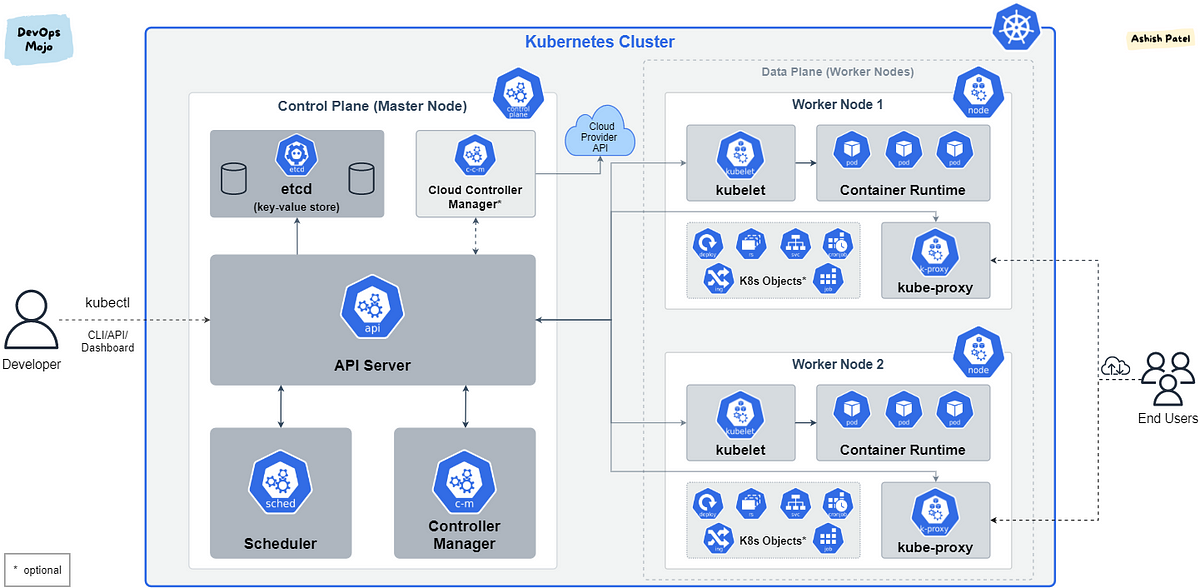
\includegraphics[width=0.85\textwidth]{figures/ch1/kubernetes_arch.png}
    \caption{Kubernetes Cluster Architecture}
    \label{fig:kube-arch}
\end{figure}

\subsection{Control Plane}
The control plane manages the data plane through the \textbf{API server}, which connects to the worker nodes via \textbf{gRPC}. Internally, the state of the nodes is updated with messages from the Kubelet and stored in \textbf{etcd}: a distributed key-value store. The control plane uses the \textbf{kube-scheduler} to select the most suitable node for the workload. Factors considered include:
\begin{itemize}
    \item \textbf{Workload constraints}: Applications can influence node selection by specifying host constraints and resource requirements.
    \item \textbf{Cluster state}: The scheduler balances resource utilization across worker nodes and avoids assigning pods to unhealthy nodes.
\end{itemize}

\subsection{Data Plane}
The data plane consists of worker nodes that execute workloads commissioned by the master in the form of pods. A pod is a group of containers managed atomically. Each worker node has two main components:
\begin{itemize}
    \item \textbf{Kubelet}: An agent that interfaces with the control plane, manages host resources, and interacts with the \textbf{Container Runtime Interface (CRI)}, which abstracts the container creation technology. In this project, all experiments use containers executed through \textbf{containerd}.
    \item \textbf{Kube-proxy}: A component that manages network traffic for the applications.
\end{itemize}

\subsubsection{Kubelet: Control Cycle}
The Kubernetes control plane continuously monitors the cluster state to ensure it matches the user's desired state. When an external modification or a node event occurs, the control plane calculates the \textbf{mutations} needed to reach the target state. These mutations are sent to the Kubelet, which translates them into pod actions.

The Kubelet operates by running a synchronization loop that processes updates from three channels (\cref{fig:worker-node}):
\begin{itemize}
    \item Configuration files;
    \item HTTP requests;
    \item API server (requests from the control plane).
\end{itemize}

\begin{figure}[htbp]
    \centering
    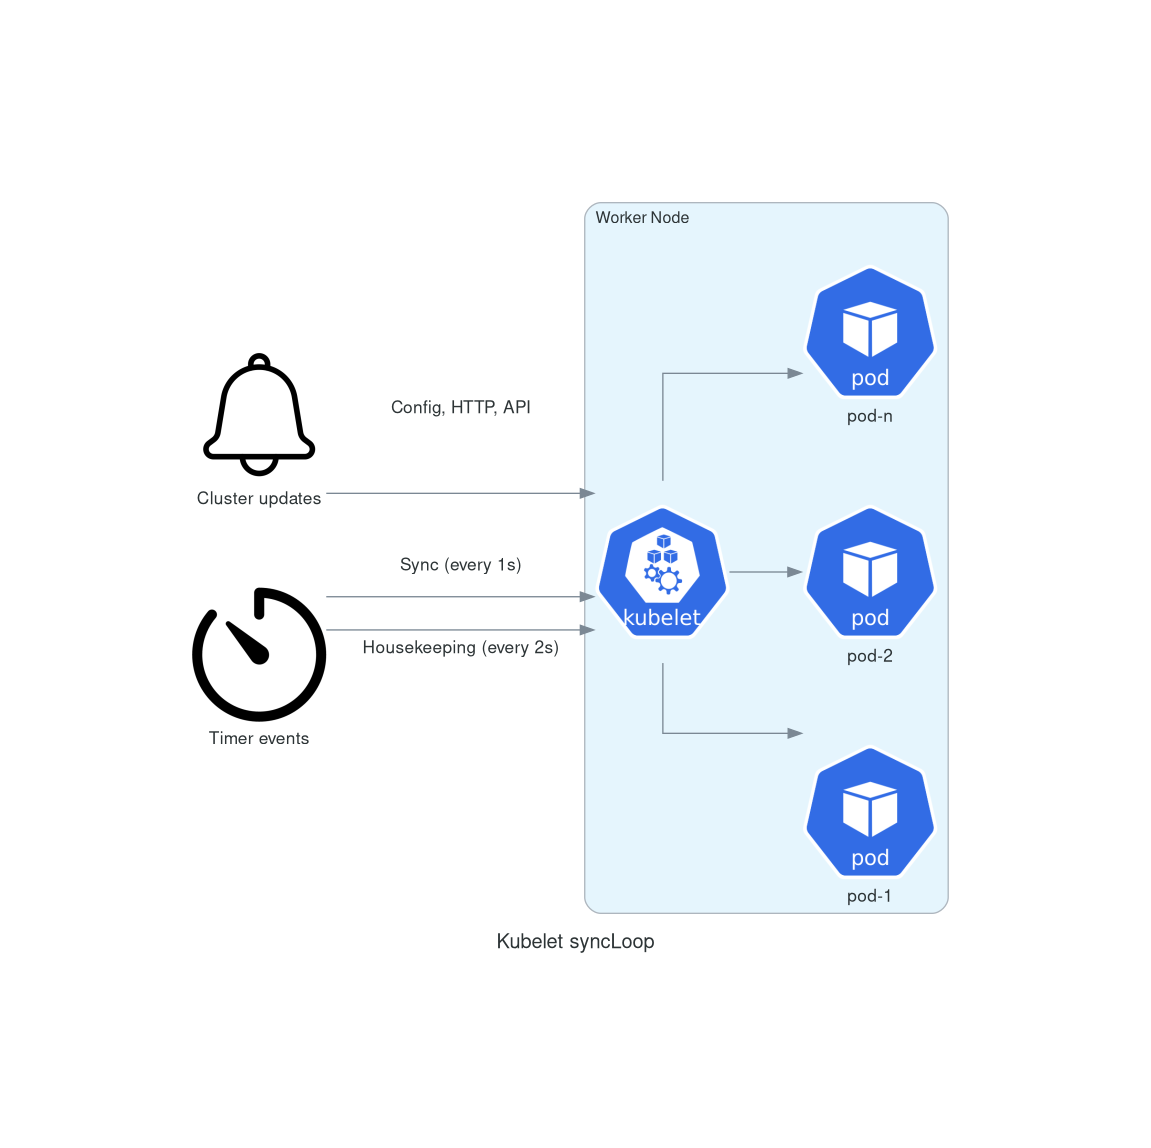
\includegraphics[width=0.85\textwidth]{figures/ch1/kubelet_syncloop.png}
    \caption{Worker Node Structure in Kubernetes}
    \label{fig:worker-node}
\end{figure}

Additionally, the Kubelet performs periodic checks every second to ensure the current state matches the desired state (\cref{fig:syncloop}). The signature of the main synchronization method is shown below:

\begin{lstlisting}[language=Go, frame=none, numbers=none, backgroundcolor=\color{white}]
func (kl *Kubelet) syncLoop(ctx context.Context, 
        updates <-chan kubetypes.PodUpdate, 
        handler SyncHandler) 
\end{lstlisting}

The three input parameters are:
\begin{itemize}
    \item \lstinline[language=Go]{type Context interface}: Contains a Deadline, a cancellation channel, errors, and user-defined values.
    \item \lstinline[language=Go]{type PodUpdate struct}: Contains a vector of pods to update, the operation type, and the update name.
    \item \lstinline[language=Go]{type SyncHandler interface}: Defines methods for handling deletion, reconfiguration, pod addition, etc.
\end{itemize}

\begin{figure}[htbp]
    \centering
    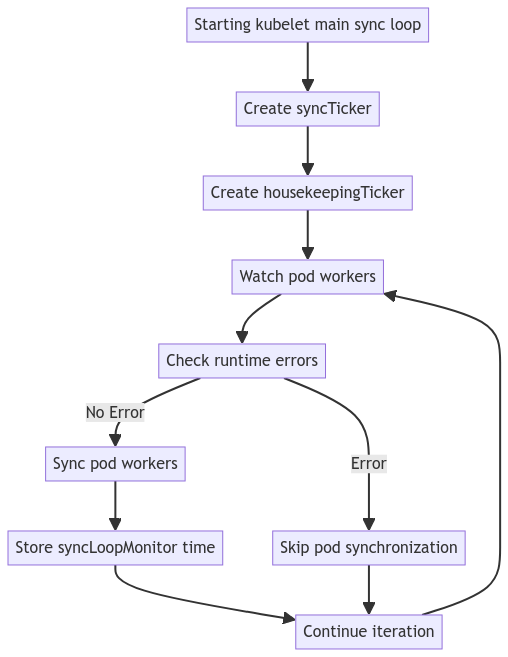
\includegraphics[width=0.6\textwidth]{figures/ch1/kubelet.png}
    \caption{syncLoop Function Flowchart}
    \label{fig:syncloop}
\end{figure}

\subsubsection{Kubelet in Linux}
The Kubelet controls hardware resources using \textbf{cgroups}. A cgroup is an isolation mechanism that limits and monitors the resources used by a group of processes. The Kubelet partitions host resources into three groups:
\begin{itemize}
    \item \textbf{kubepods}: Resources dedicated to pods.
    \item \textbf{system-resources}: Used for processes not belonging to Kubernetes.
    \item \textbf{kube-resources}: Resources allocated for Kubernetes-related processes on the host, such as the container runtime and the Kubelet itself.
\end{itemize}
Pod resources are further grouped into three Quality of Service (QoS) classes: \textbf{Guaranteed}, \textbf{Burstable}, and \textbf{Best Effort}.

\begin{center}
\begin{forest}
  for tree={
    font=\ttfamily\small,
    grow'=0,
    child anchor=west,
    parent anchor=south,
    anchor=west,
    calign=first,
    edge path={
      \noexpand\path [draw, \forestoption{edge}]
      (!u.south west) +(7.5pt,0) |- node[fill,inner sep=1.25pt] {} (.child anchor)\forestoption{edge label};
    },
    before typesetting nodes={
      if n=1
        {insert before={[,phantom]}}
        {}
    },
    fit=band,
    before computing xy={l=15pt},
  }
[/sys/fs/cgroup/
  [kubepods/
    [besteffort/
        [<container\_id>/]
    ]
    [burstable/
        [<container\_id>/]
    ]
     [guaranteed/
        [<container\_id>/]
    ]
  ]
  [system-resources/
  ]
  [kube-resources/]
]
\end{forest}
\end{center}

\subsection{Containers in Linux} \label{section:linux_container}
A container is an isolated application based on kernel sharing, making it highly efficient to manage. To ensure decoupling, the Kubelet does not interact directly with the kernel to create containers. Instead, it uses the \textbf{Container Runtime Interface (CRI)}, as shown in \cref{fig:kubelet_2_containerd}.

\begin{figure}[htbp]
    \centering
    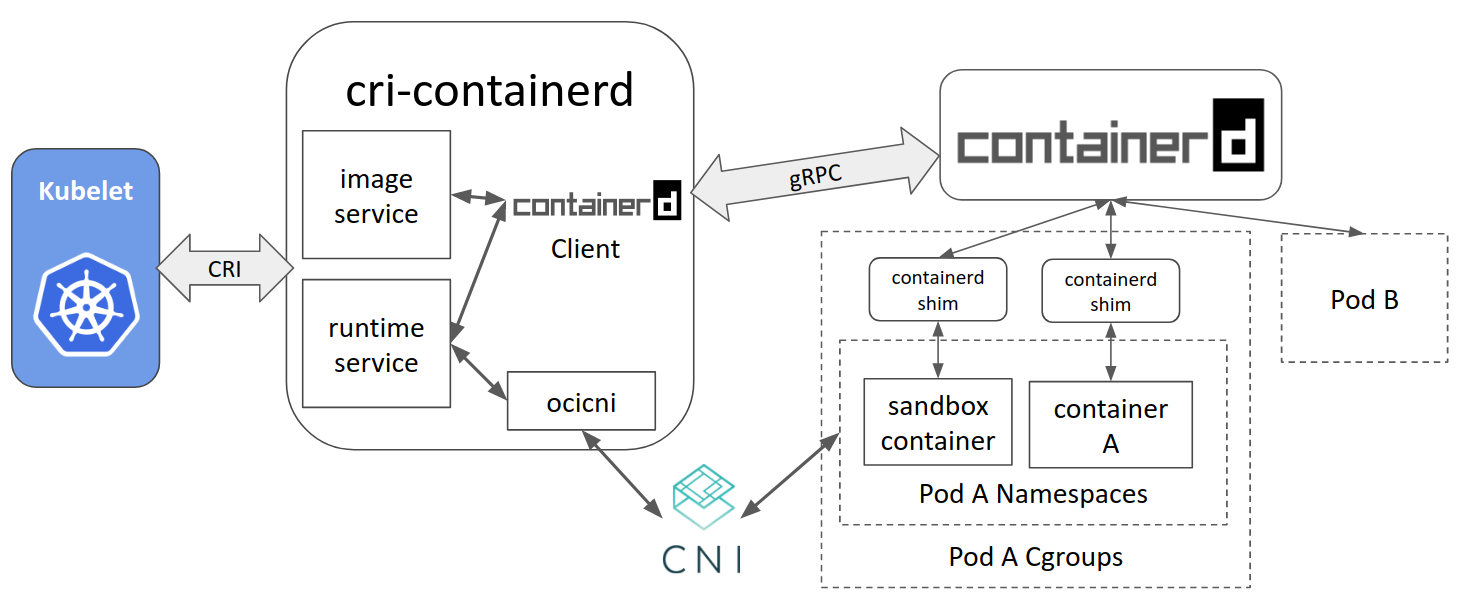
\includegraphics[width=0.75\textwidth]{figures/ch1/containerdimg.png}
    \caption{Interaction Architecture between containerd and Kubelet}
    \label{fig:kubelet_2_containerd}
\end{figure}

In this project, the container runtime is \textbf{containerd}. Specifically, the Kubelet uses a component called \textbf{cri-containerd} to interact with containerd via \textbf{gRPC} APIs. As shown in \cref{fig:kubelet_2_containerd}, managing a pod with $n$ containers involves creating $n+1$ containers because the Kubelet requires a special container called the \textbf{Sandbox}, which uses the \textbf{pause} image. This assembly-based application maintains the pod's \textbf{network namespace}~\cite{WhatIsPauseContainer}. Linux namespaces are deleted when no processes remain in them; thus, the pause container prevents downtime during container replacement~\cite{WhyPauseContainer, ManUnshare}.

\paragraph{Containerd} Containerd~\cite{Containerd} is a high-level container runtime written in Go. It manages the container lifecycle by communicating with a low-level container runtime. This abstraction, based on the \textbf{OCI}~\cite{OpenContainerInitiative} standard, separates container implementation from usage. Containerd uses \textbf{runc} as its default low-level runtime.

\paragraph{Runc} Runc creates containers using Linux system calls, configuring them through namespaces and virtual file I/O. The creation process involves a double \textit{fork} (using \textbf{clone} and \textbf{unshare}): the first creates the container process, while the second ensures the container is not terminated if runc exits, and vice versa.

Listing~\ref{lst:runc_config} shows an example of high-level container configuration in Go.

\begin{lstlisting}[language=Go, label=lst:runc_config, caption={High-level Container Configuration Example}]
config := &configs.Config{
	Rootfs: "/your/path/to/rootfs",
	Capabilities: &configs.Capabilities{
		Bounding: []string{
			"CAP_KILL",
			"CAP_AUDIT_WRITE",
		},
	},
	Namespaces: configs.Namespaces([]configs.Namespace{
		{Type: configs.NEWNS},
		{Type: configs.NEWUTS},
		{Type: configs.NEWIPC},
		{Type: configs.NEWPID},
		{Type: configs.NEWUSER},
		{Type: configs.NEWNET},
		{Type: configs.NEWCGROUP},
	}),
	Cgroups: &configs.Cgroup{
		Name:   "test-container",
		Parent: "system",
		Resources: &configs.Resources{
			MemorySwappiness: nil,
			Devices:          devices,
		},
	},
	MaskPaths: []string{
		"/proc/kcore",
		"/sys/firmware",
	},
	ReadonlyPaths: []string{
		"/proc/sys", "/proc/sysrq-trigger", "/proc/irq", "/proc/bus",
	},
	Devices:  specconv.AllowedDevices,
	Hostname: "testing",
	Mounts: []*configs.Mount{
		{
			Source:      "proc",
			Destination: "/proc",
			Device:      "proc",
			Flags:       defaultMountFlags,
		},
	},
	UIDMappings: []configs.IDMap{
		{
			ContainerID: 0,
			HostID: 1000,
			Size: 65536,
		},
	},
	GIDMappings: []configs.IDMap{
		{
			ContainerID: 0,
			HostID: 1000,
			Size: 65536,
		},
	},
	Networks: []*configs.Network{
		{
			Type:    "loopback",
			Address: "127.0.0.1/0",
			Gateway: "localhost",
		},
	},
	Rlimits: []configs.Rlimit{
		{
			Type: unix.RLIMIT_NOFILE,
			Hard: uint64(1025),
			Soft: uint64(1025),
		},
	},
}
\end{lstlisting}

The \textbf{nsexec} function is critical for container creation. Key system calls used include:
\begin{itemize}
    \item \lstinline{clone()}: Creates a new process with controlled namespaces and address space~\cite{ManClone}.
    \item \lstinline{unshare()}: Allows a process to disassociate parts of its execution context~\cite{ManUnshare}.
    \item \lstinline{pivot_root()}: Changes the root directory for the calling process.
    \item \lstinline{setns()}: Associates the calling process with a specified namespace~\cite{ManSetns}.
    \item \lstinline{mount()}: Mounts a filesystem.
    \item \lstinline{execve()}: Executes the specified command.
\end{itemize}

\section{Pod Creation Latency Analysis}

\subsection{Problem Statement}
The objective is to propose an upper bound (potentially theoretical) for the creation and startup time of a Kubernetes container. The focus is on the Kubelet-generated latency (\cref{fig:pod_latency}, green section), which depends on the worker node and the container technology.

\begin{figure}[htbp]
    \centering
    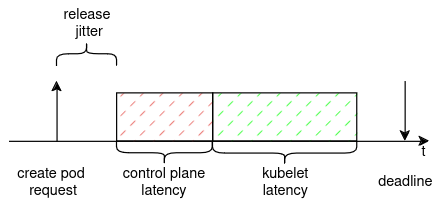
\includegraphics[width=0.65\textwidth]{figures/ch1/latency.png}
    \caption{Pod Creation Timing Diagram}
    \label{fig:pod_latency}
\end{figure}

\paragraph{Why is Kubernetes unsuitable for hard real-time tasks?} Kubernetes and containerd are written in Go~\cite{Golang}, a high-level, garbage-collected language. While the garbage collector can be disabled~\cite{GoGarbageCollector} and manual allocation performed via CGO, the Go runtime uses an \textbf{M:N fair scheduler}~\cite{GolangScheduler} with \textbf{work stealing}~\cite{GolangSchedulerDeepDive} and a $10ms$ time slice~\cite{GolangScheduler}. This makes Go inherently unsuitable for hard real-time applications.

\begin{figure}[htbp]
    \centering
    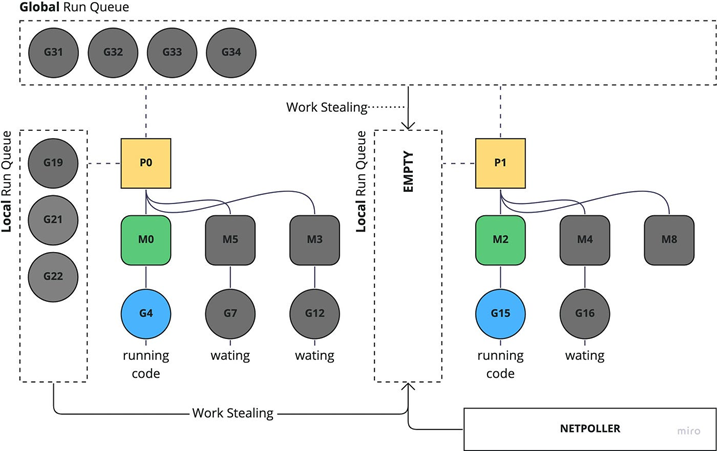
\includegraphics[width=0.65\textwidth]{figures/ch1/golang_scheduler.png}
    \caption{Goroutine Scheduling Overview}
    \label{fig:golang_scheduler}
\end{figure}

\subsection{Test Environment}
Latency analysis was conducted using a single-container \textbf{nginx} pod. The study factors are listed in \cref{tab:factor}. \textbf{SCHED\_FIFO} and \textbf{priority} refer to the containerd and Kubelet processes, while \textbf{cgroup} refers to running both in the same cgroup. 20 samples were collected for each experiment.

\begin{table}[htbp]
\centering
\small
    \begin{tabular}{ll}
    \toprule
    \textbf{Factor} & \textbf{Values} \\ \midrule
    \# pods & $5, 10, 20, 30, 40, 50$ \\
    \# CPUs & $2, 4, 8$ \\
    Scheduler & SCHED\_FIFO, SCHED\_OTHER \\
    \# Isolated CPUs & True, False \\
    Priority & $90, 99$ \\
    Cgroup & $0, 1, 2$ \\ \bottomrule
\end{tabular}
\caption{Factors Considered in Latency Analysis}
\label{tab:factor}
\end{table}

\paragraph{Assumptions} To focus on Kubelet-OS interactions:
\begin{itemize}
    \item \textbf{Local image availability}: Container images are pre-pulled to eliminate network variability.
    \item \textbf{Isolated workload}: The Kubelet is assumed to be the primary user of the worker node.
\end{itemize}

\paragraph{Setup} The test machine specifications are listed in \cref{tab:test_machine}.

\begin{table}[htbp]
\centering
\small
    \begin{tabular}{ll}
    \toprule
    \textbf{Feature} & \textbf{Test Machine} \\ \midrule
    CPU & AMD Ryzen 7, 5700U 4.3GHz \\
    RAM & DDR4 16GB, 3200 MHz SODIMM \\
    OS & Linux taurino 6.9.2-artix1-1 \#1 SMP PREEMPT\_DYNAMIC \\ \bottomrule
\end{tabular}
\caption{Test Machine Characteristics}
\label{tab:test_machine}
\end{table}

A local Kubernetes cluster was created as described in~\cite{Medium}. The etcd server was run in standalone mode, followed by the kube-controller-manager (with `kube-api-qps` set to -1 to disable rate limiting) and the API server. Containerd was configured with `systemdCgroup=false`. Finally, the Kubelet was started with JSON logging.

\paragraph{Metrics} Metrics were extracted from Kubelet logs using the \textbf{podStartE2EDuration} field, which measures end-to-end latency, including Sandbox creation.

\subsection{Results}\label{section:results}
Startup time distributions were analyzed using violin and box plots. Since the distributions are non-normal, mean values (\cref{fig:average}) are insufficient as descriptive statistics. Consequently, Extreme Value Theory (EVT)~\cite{Evt} was used to analyze tail behavior.

\begin{figure}[htbp]
    \centering
    \includegraphics[width=0.9\textwidth]{figures/ch2/results/average.pdf}
    \caption{Average Pod Startup Times for $n$ Pods}
    \label{fig:average}
\end{figure}

The operating system \textbf{scheduler} is the most significant factor. \cref{fig:fifo-vs-nofifo} shows that \textbf{SCHED\_FIFO} drastically reduces latency compared to \textbf{SCHED\_OTHER}, which exhibits a wider interquartile range.

\begin{figure}[htbp]
    \centering
    \begin{subfigure}{0.48\textwidth}
        \includegraphics[width=\linewidth]{figures/ch2/results/cgroup-fifo-k90-c99.box.pdf}
        \caption{SCHED\_FIFO (Priority 90)}
    \end{subfigure}\hfill
    \begin{subfigure}{0.48\textwidth}
        \includegraphics[width=\linewidth]{figures/ch2/results/cgroup-nort.box.pdf}
        \caption{SCHED\_OTHER (No cgroup)}
    \end{subfigure} \\
    \begin{subfigure}{0.48\textwidth}
        \includegraphics[width=\linewidth]{figures/ch2/results/nocgroup-4cpu-fifo-k99-c99.box.pdf}
        \caption{SCHED\_FIFO (4 CPUs, No cgroup)}
    \end{subfigure}\hfill
    \begin{subfigure}{0.48\textwidth}
        \includegraphics[width=\linewidth]{figures/ch2/results/2cgroup-4cpu-fifo-k99-c99.box.pdf}
        \caption{SCHED\_FIFO (4 CPUs, 2 cgroups)}
    \end{subfigure}
    \caption{Latency Results for Various Cgroup and Scheduler Configurations}
    \label{fig:fifo-vs-nofifo}
\end{figure}

Violin plots (\cref{fig:fifo-vs-nofifo-violin}) confirm that SCHED\_OTHER values cluster toward the maximum, while SCHED\_FIFO values cluster toward the minimum with lower variance.

\begin{figure}[htbp]
    \centering
    \begin{subfigure}{0.48\textwidth}
        \includegraphics[width=\linewidth]{figures/ch2/results/cgroup-fifo-k90-c99.violin.pdf}
        \caption{SCHED\_FIFO (Priority 90)}
    \end{subfigure}\hfill
    \begin{subfigure}{0.48\textwidth}
        \includegraphics[width=\linewidth]{figures/ch2/results/cgroup-nort.violin.pdf}
        \caption{SCHED\_OTHER (No cgroup)}
    \end{subfigure} \\
    \begin{subfigure}{0.48\textwidth}
        \includegraphics[width=\linewidth]{figures/ch2/results/nocgroup-4cpu-fifo-k99-c99.violin.pdf}
        \caption{SCHED\_FIFO (4 CPUs, No cgroup)}
    \end{subfigure}\hfill
    \begin{subfigure}{0.48\textwidth}
        \includegraphics[width=\linewidth]{figures/ch2/results/2cgroup-4cpu-fifo-k99-c99.violin.pdf}
        \caption{SCHED\_FIFO (4 CPUs, 2 cgroups)}
    \end{subfigure}
    \caption{Violin Plots for Cgroup and Scheduler Variants}
    \label{fig:fifo-vs-nofifo-violin}
\end{figure}

Increasing CPU count with real-time scheduling shows limited benefit from cgroup isolation (\cref{fig:fifo-nocgroup-box}). However, exclusive CPU allocation via `isolcpus`~\cite{IsolCPU} yields excellent results by eliminating OS housekeeping overhead (\cref{fig:fifo-isolcpus}).

\begin{figure}[htbp]
    \centering
    \begin{subfigure}{0.48\textwidth}
        \includegraphics[width=\linewidth]{figures/ch2/results/nocgroup-4cpu-fifo-k99-c99.box.pdf}
    \end{subfigure}\hfill
    \begin{subfigure}{0.48\textwidth}
        \includegraphics[width=\linewidth]{figures/ch2/results/nocgroup-8cpu-fifo-k99-c99.box.pdf}
    \end{subfigure}\\
    \begin{subfigure}{0.48\textwidth}
        \includegraphics[width=\linewidth]{figures/ch2/results/nocgroup-4cpu-fifo-k99-c99.violin.pdf}
        \caption{SCHED\_FIFO (4 CPUs)}
    \end{subfigure}\hfill
    \begin{subfigure}{0.48\textwidth}
        \includegraphics[width=\linewidth]{figures/ch2/results/nocgroup-8cpu-fifo-k99-c99.violin.pdf}
        \caption{SCHED\_FIFO (8 CPUs)}
    \end{subfigure}
    \caption{Startup Trends with SCHED\_FIFO and Varying CPU Counts (No Cgroup)}
    \label{fig:fifo-nocgroup-box}
\end{figure}

\begin{figure}[htbp]
    \centering
    \begin{subfigure}{0.48\textwidth}
        \includegraphics[width=\linewidth]{figures/ch2/results/nocgroup-2-isolcpus-fifo-k99-c99.violin.pdf}
    \end{subfigure}\hfill
    \begin{subfigure}{0.48\textwidth}
        \includegraphics[width=\linewidth]{figures/ch2/results/nocgroup-2-isolcpus-fifo-k99-c99.box.pdf}
    \end{subfigure}
    \caption{Startup Trends with Isolated CPUs}
    \label{fig:fifo-isolcpus}
\end{figure}

\subsubsection{Extreme Value Analysis of End-to-End Pod Creation Time}
EVT~\cite{Evt} estimates probabilistic Worst-Case Execution Time (WCET) by focusing on tail events. It requires three hypotheses: \textbf{stationarity}, \textbf{short-range independence}, and \textbf{long-range independence}. Converging maxima follow the \textbf{Generalized Extreme Value (GEV)} distribution (\cref{eq:gev}).

\begin{equation}
    F(x) = \exp{\left(-\left(1 + \xi \frac{x-\mu}{\sigma}\right)^{-\frac{1}{\xi}}\right)}
    \label{eq:gev}
\end{equation}

SCHED\_FIFO experiments provided the best fits (\cref{tab:fit_data}), often resulting in a \textbf{Weibull} distribution ($\xi < 0$), commonly used for reliability modeling~\cite{WeibullUses}.

\begin{table}[htbp]
\centering
\small
    \begin{tabular}{lc}
    \toprule
    \textbf{Experiment} & \textbf{$\xi$} \\ \midrule
    2cgroup-4cpu-fifo-k99-c99 & -0.023 \\
    nocgroup-8cpu-fifo-k99-c99 & -0.43 \\
    cgroup-fifo-k90-c99 & 0.25 \\
    nocgroup-2-isolcpus-fifo-k99-c99 & 1.08 \\ \bottomrule
    \end{tabular}
\caption{GEV Fit Shape Parameters ($\xi$) for Key Experiments}
\label{tab:fit_data}
\end{table}

\begin{figure}[htbp]
    \centering
    \includegraphics[width=0.9\textwidth]{figures/ch2/evt/qqplot-2cgroup-4cpu-fifo-k99-c99.pdf}
    \caption{QQ Plots for Selected GEV-Fitted Experiments}
    \label{fig:variance}
\end{figure}

\section{Upper Bound on Pod Startup Time}
\subsection{Theoretical Model for Pod Startup Time}
Kubernetes can be modeled as a mixed-criticality system. Total latency $L_{pod}$ is:
\begin{equation*}
    L_{pod}(S) = L_{cp}(S_{cp}) + L_{wn}(S_{wn}) + \delta
\end{equation*}
where $L_{cp}$ is control plane latency, $L_{wn}$ is worker node latency, and $\delta$ is network overhead. This analysis focuses on $L_{wn}(S_{wn})$. The primary latency contributors are (\cref{fig:latency-detail}):
\begin{enumerate}
    \item $t_w$: Queuing time at the worker node.
    \item $t_i$: Image preparation.
    \item $t_{runc}$: System call execution by runc.
\end{enumerate}

\begin{figure}[htbp]
    \centering
    
\includegraphics[width=0.7\textwidth]{figures/ch3/latency.png}
    \caption{Detailed Worker Node Latency Breakdown}
    \label{fig:latency-detail}
\end{figure}

\begin{equation}
    L_{wn}(S_{wn}) =  t_w(S_{wn}) +  t_i(S_{wn}) + t_{runc}(S_{wn})
    \label{eq:pod_latency}
\end{equation}

\subsubsection{Analysis of $t_i(S_{wn})$}
Image preparation involves filesystem and network operations:
\begin{equation*}
    t_i = \begin{cases}
    c & \text{if image is locally present} \\
    t_d + c & \text{otherwise}
    \end{cases}
\end{equation*}
Pre-tagging images in containerd ensures $t_i = c$.

\subsubsection{Analysis of $t_{runc}(S_{wn})$}
Based on \textit{nsexec.c}~\cite{Runc}, container creation requires 11 system calls. For a single-container pod:
\begin{equation*}
    t_{runc}(S_{wn}) = 2 \cdot m \cdot \max (T_{sys})
\end{equation*}
where $m=11$ and $T_{sys}$ is the system call execution time.

\subsubsection{Analysis of $t_w(S_{wn})$}
Bounding $t_w$ requires rate limiting and scheduling modifications.

\paragraph{Rate Limiting: Fixed Window Algorithm}
Limits requests within a predefined timeframe (\cref{fig:fixed_window})~\cite{FixedWindowAlgorithm}.

\begin{figure}[htbp]
\centering
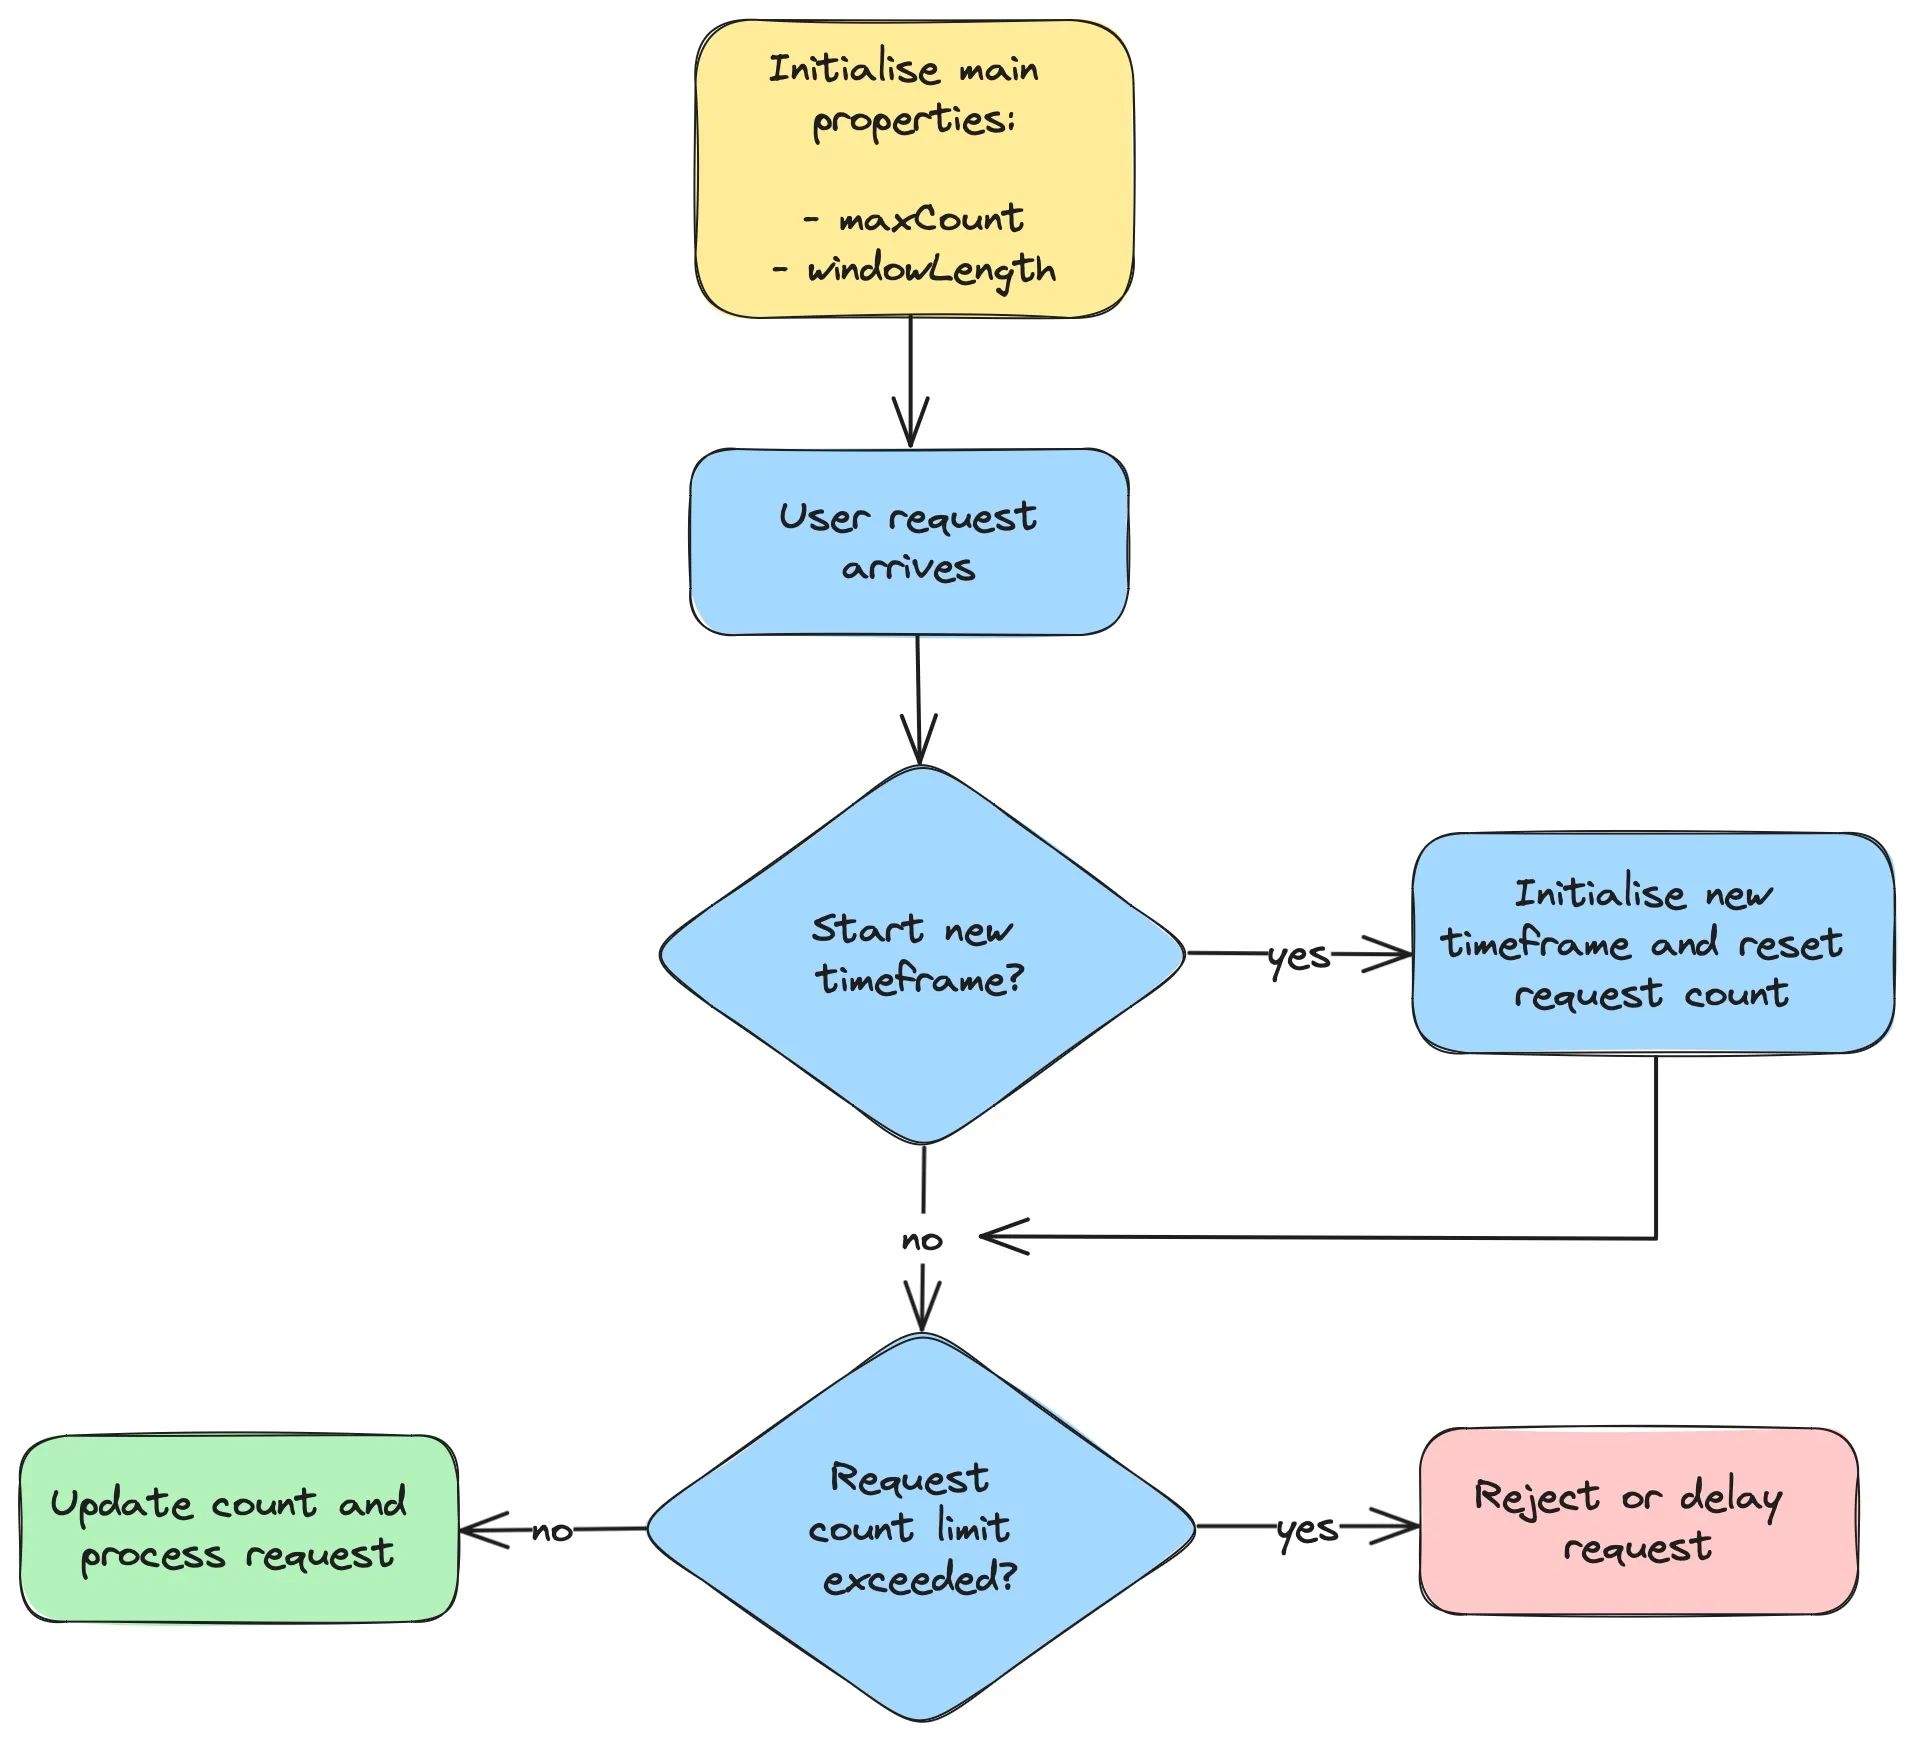
\includegraphics[width=0.7\textwidth]{figures/ch3/fixed_window.png}
\caption{Fixed Window Algorithm Flowchart}
\label{fig:fixed_window}
\end{figure}

\paragraph{Scheduling: Deferrable Server}
A deferrable server provides a theoretical schedulability test to guarantee deadlines.
\begin{equation*}
    U_p \leq n \left[\left(\frac{U_s + 2}{2U_s + 1}\right)^{1/n} - 1\right]
\end{equation*}

This approach is compatible with the SCHED\_FIFO rate-monotonic scheduler in the Linux kernel.

\clearpage
\addcontentsline{toc}{section}{References}
\bibliographystyle{plain}
\bibliography{refs}
\end{document}
